\documentclass[12 pt]{article}
%\usepackage[a4paper,top=4cm,bottom=3.5cm,left=3.5cm,right=3.5cm]{geometry}
\usepackage{graphicx} 
\usepackage{amssymb}
\usepackage{lmodern}
\usepackage{amsmath}
\usepackage{hyperref}
\usepackage{footnotebackref}
\newcommand\tab[1][1cm]{\hspace*{#1}}
\usepackage{setspace}
\author{Vanessa Braglia}
\title{The swiss scientific social network}
\date{\today}

%\onehalfspacing

\begin{document}
\fontfamily{lmr}\selectfont
\maketitle 
\newpage
\tableofcontents
\newpage
\section{Introduction}
A social network consists of a set of objects connected to each other by social relations. The best way to model social networks is using graphs (see an example in Figure 1): the objects (entities) are represented as nodes and the connections as edges between two different nodes. The most common example we can take is the World Wide Web (WWW) where we have web pages as nodes connected by hyperlinks, the edges.\\
\begin{figure} [h!]
\centering 
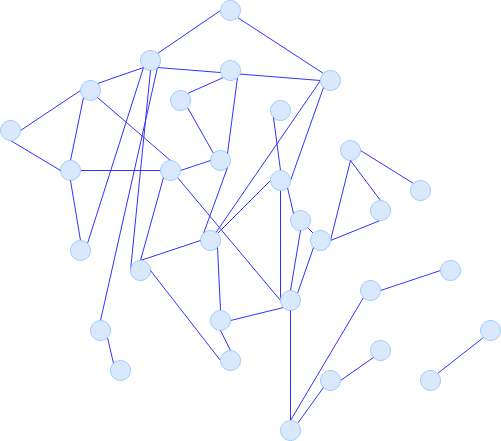
\includegraphics[scale=0.3]{./img/graph3.png}
\caption{Example of social network graph}
\end{figure}
\\
The goal of this project is to create a social network of computational science authors belonging to Swiss institutions and then analyze the relative graph.\\
The first step is retrieving all necessary information for the construction of the social network: names of the authors and relationships between each other. I crawled the 2015,2016 and 2017 PASC Conferences, interdisciplinary conferences which brings together research across the areas of computational science, high-performance computing, and various domain sciences, and SIAM conferences of several years, selecting the topics relevant to us (e.g. Optimization, Parallel Computing,...). \\
The second step is the information analysis to find out relations between institutions but also between members belonging to the same institution.\\
With PageRank algorithm we obtain a ``ranking" of all conferences' participants: PageRank is an algorithm used by Google Search to rank websites in their search engine results but it can be applied to any social network. In this project I use the algorithm to measure the importance of institutions' members considering the number and quality of their collaborations.\\
I use Graph Partitioning to ``invert" the process and obtain the institutions from members collaborations: probably members of the same institution collaborate more between each other than with other institutions' representatives.\\
I also analyze the institutions' connectivity matrices and their structure: looking at the cliques (i.e. a sub matrix where every two distinct members collaborate with each other; this means that all entries of the sub matrix are ones) present in the matrices we can for example detect the different research areas of the institutions and the connection between them.\\
The results will provide an interesting picture of the different research scenarios in Switzerland and how they interact with each other.

\section{PageRank Algorithm}
PageRank is an algorithm used by Google Search to rank websites in their search engine results; it was developed by  Larry Page and  Sergey Brin (the two founders of Google) in 1996 as part of their research project at Stanford University. \\
PageRank is used, together with other algorithms, to measure the importance of web pages and sort them by popularity in the result; it can be used in any graph to compute the importance of each node with its PageRank value. Larry Page and  Sergey Brin algorithm works by counting the number and quality of links to a page to compute a value which represents its importance; more popular a page is, more likely it receives links from other websites and more likely from important websites.\\
\begin{figure}[h!]
\begin{center}
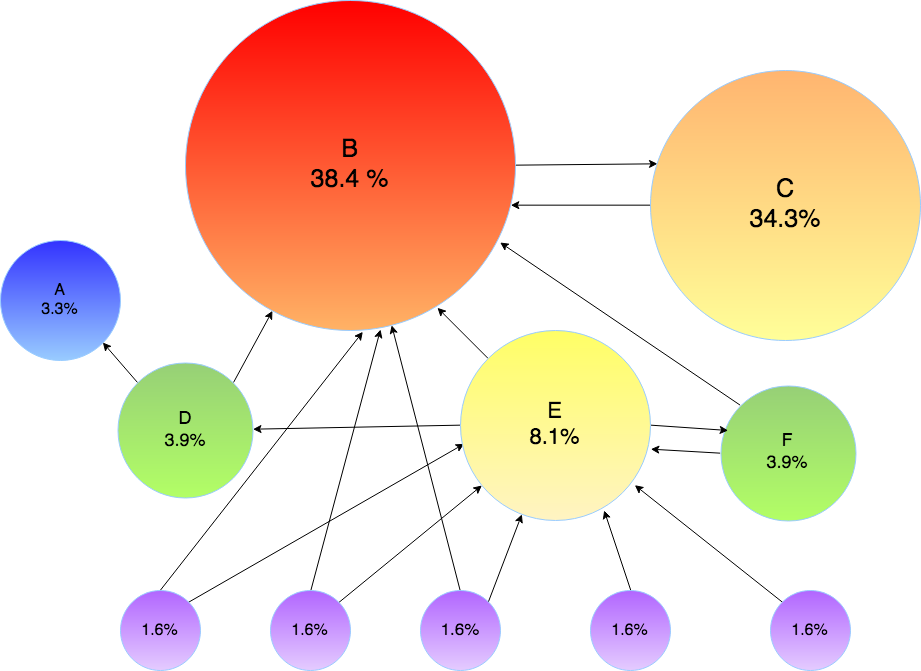
\includegraphics[scale=0.3]{./img/page_rank_example.png}
\caption{PageRank example}
\end{center}
\end{figure}
As we can see in Figure 2, node C has higher PageRank than E even if it has lower number of inner links; this is because the only inner link C has is from the most important node of the graph B so it is considered more than all the inner links of E from purple lower nodes.

Imagine surfing websites, going from one page to another: to avoid problems with pages without outer links we have two different methods to choose the next page. Our surfer can:
\begin{itemize}
\item randomly choose an outgoing link from the page,
\item simply choose a random page from the Web.
\end{itemize}
We assume that with probability $p$ (typically p=0.85) our surfer follows the first option and with probability $1-p$ the second.\\
The probability that an infinite random surfer visits a specific website it's called its PageRank; a page will have high rank if other pages with high rank link to it.
\subsection{How to compute PageRank values?}
To apply PageRank, from a graph of $n$ nodes we construct a $n$-by-$n$ connectivity matrix G: $g_{ij}=1$ if and only if node i and j are connected. The number of non-zeros in G is the total number of connections in the graph.\\
The row $r_i$ represents the number of inner-links of page $i$, instead column $c_i$ the number of outer-links. So we can define:
\begin{itemize}
\item In-degree of page $i$: \tab $r_i = \sum\limits_{j=1}^{n} g_{ij}$
\item Out-degree of page $i$: \tab $c_i = \sum\limits_{j=1}^{n} g_{ji}$
\end{itemize}
Let $p$ be the probability that the surfer follows a link and $1-p$ the probability that it chooses a random page. \\
$\delta = \frac{1-p}{n}$ is the probability that a particular random page is chosen.\\
We construct a transition probability matrix A where all elements are positive, smaller than one and sums of columns are equal to one; column $j$ represents the probabilities to go from page j to all other pages. So we set:\\
\begin{equation}\notag
a_{ij} = 
\begin{cases}
\frac{pg_{ij}}{c_{j}} + \delta  & \text{if } c_{j} \neq 0\\
\frac{1}{n} & \text{if } c_{j} = 0
\end{cases}
\end{equation}
If the page $j$ has no outer links it means that column $j$ of A assigns equal probability $\frac{1}{n}$ to all its elements.\\
We can now compute PageRanks values solving the homogeneous linear system:
$$x = A\:x$$
The transition matrix A can be written as
$$A = pGD+ez^{T}$$
where D is a diagonal matrix with the reciprocals of the out-degrees
\begin{equation}\notag
d_{jj} = 
\begin{cases}
\frac{1}{n} & \text{if } c_{j} \neq 0\\
0 & \text{if } c_{j} = 0
\end{cases}
\end{equation}
z is the vector formed by
\begin{equation}\notag
z_{j} = 
\begin{cases}
\delta & \text{if } c_{j} \neq 0\\
\frac{1}{n} & \text{if } c_{j} = 0
\end{cases}
\end{equation}
and e is the vector of length n with all ones.\\
We can write the linear system
$$(I-A)x=0$$
as
$$(I - pGD)x = \gamma e$$
where we take $\gamma = z^{T} x=1$. WHY?\\
To conclude, we find the solution of
$$(I - pGD)x = e$$
and then rescale the solution x so that $\sum\limits_{i=1}^{n} x_i = 1$.
\subsubsection{PageRank algorithm}
\begin{center}
\framebox[\textwidth][l]{\parbox{\textwidth}{
\textbf{Input}: a list of authors U, the corresponding adjacency matrix G \\
\tab \tab and a damping factor p\\
\textbf{Output}: list of authors sorted according to PageRank in descending order\\
\begin{itemize}
\item[1.] Remove self collaborations \tab $G = G - diag(G)$
\item[2.] Compute out-degree and in-degree of each node \\
$c = sum(G,1)$ and  $r = sum(G,2)$
\item[3.] Create diagonal matrix D with the reciprocals of the out-degrees
\item[4.] Solve $(I - pGD)x = e$
\item[5.] Normalize the result x \tab $x = x/sum(x)$
\item[6.] Sort x in descending order
\end{itemize}
}}
\end{center}
\section{Graph Partitioning}
Graph partitioning consists in dividing a graph $G=(V,E)$\footnote{A graph G with vertexes V and edges E.}  cutting the smaller number of edges and obtaining sub-graphs with specific properties. For example k-way partitioning divides the graph G into k smaller components.\\
To apply graph partitioning we need the adjacency matrix A of the graph, which is symmetric, and the Laplacian matrix L constructed such that:
\begin{equation}\notag
L_{ij} = 
\begin{cases}
d_i \tab if i=j \\
-1 \tab if i \neq j \:\: and \: \: (i,j) \in E \\
0 \tab \text{otherwise}
\end{cases}
\end{equation}
where $d_i$ is the vertex degree of node $i \in V$.\\
The relation between A and L is
$$L = D - A$$
where D is the diagonal matrix where $d_{ii}$ if the vertex degree of node $i \in V$.\\
Since L is symmetric and positive semidefinite per construction, all its eigenvalues are real and nonnegative. The first eigenvalue is always zero and the second is not equal to zero if the graph is connected\footnote{there is a path from any node to any other node in the graph}; we can define eigenvalues of L as follows
$$ 0 = \lambda1 < \lambda_2 \leq ... \leq \lambda_n$$
The eigenvector corresponding to the first eigenvalue $\lambda_1$ is the vector of all ones and it does not provide information about the graph structure; instead the second lowest eigenvector, Fiedler vector, is used by spectral partitioning to return the smaller sub-graphs. Dividing the nodes of graph G according to the median $s$ of the Fiedler vector $\vec{v} = (v_1,v_2,...,v_n)$ helping obtaining two partitions $V_1$ and $V_2$:
\begin{equation}\notag
\begin{cases}
v_i \in V_1 \Longrightarrow v_i \leq s \\
v_i \in V_2 \Longrightarrow v_i > s
\end{cases}
\end{equation}
Such a partition is called the Fiedler cut and leads to two parts of G with nearly equals number of vertexes with small number of cutting edges.
\subsubsection{Spectral partitioning algorithm}
\begin{center}
\framebox[\textwidth][l]{\parbox{\textwidth}{
\textbf{Input}: a graph $G=(V,E)$ \\
\textbf{Output}: two graphs $G_1=(V_1,E_1)$ and $G_2=(V_2,E_2)$ \\
\begin{itemize}
\item[1.] Compute Fiedler vector of L = D - A 
\item[2.] Sort the vector values 
\item[3.] Put first half of the nodes in $V_1$ 
\item[4.] Put second half of the nodes in $V_2$ 
\item[5.] $E_1$ be the set of edges with both nodes in $V_1$ 
\item[6.] $E_2$ be the set of edges with both nodes in $V_2$
\end{itemize}
}}
\end{center}
\subsection{K-way Partitioning}
K-way partitioning of a graph G of n nodes, consists in a division of its nodes in k disjoint subset, all with size nearly $\frac{n}{k}$.\\
We consider only the simple case where we want to divide the graph in k partitions and k is a power of two. The idea is just to apply the spectral partitioning $\frac{k}{2}$ times recursively.
\subsubsection{Recursive Spectral partitioning algorithm}
\begin{center}
\framebox[\textwidth][l]{\parbox{\textwidth}{
\textbf{Input}: a graph $G=(V,E)$ and number $k$ of desired partitions\\
\textbf{Output}: $k$ graphs $G_1=(V_1,E_1)$ ... $GK=(V_K,E_K)$ \\
\begin{itemize}
\item[1.] Apply spectral partitioning on G to find $G_1$ and $G_2$
\item[2.] If $\frac{k}{2} > 1$
\begin{itemize}
\item[2.1] recursive partition on $G_1$ with $\frac{k}{2}$
\item[2.2] recursive partition on $G_2$ with $\frac{k}{2}$
\item[2.3] $k = \frac{k}{2}$
\end{itemize}
\item[3.] Return partitions $G_1$ ... $G_K$
\end{itemize}
}}
\end{center}
\section{Results}
Cliques\footnote{Some text in a footnote.}
\subsection{Information Retrieval}
\subsection{PageRank}
\subsection{Graph Partitioning}
\section{Bibliography}
\begin{itemize}
\item https://en.wikipedia.org/wiki/PageRank
\item Assignment1 1 Course Numerical Computing 2107/2018
\item Assignment2 1 Course Numerical Computing 2107/2018
\item \hyperref[label_name]{''https://am.vsb.cz/export/sites/am/cs/theses/kabelikova\_ing.pdf''}
\end{itemize}
\end{document}
